\documentclass[portrait,final]{baposter}
%\documentclass[a4shrink,portrait,final]{baposter}
% Usa a4shrink for an a4 sized paper.

\tracingstats=2

\usepackage{times}
\usepackage{calc}
\usepackage{graphicx}
\usepackage{amsmath}
\usepackage{amssymb}
\usepackage{relsize}
\usepackage{multirow}
\usepackage{bm}

\usepackage{graphicx}
\usepackage{wrapfig}
\usepackage{multicol}

\usepackage{pgfbaselayers}
\pgfdeclarelayer{background}
\pgfdeclarelayer{foreground}
\pgfsetlayers{background,main,foreground}

\usepackage{helvet}
%\usepackage{bookman}
\usepackage{palatino}

\usepackage{url}
\usepackage{fancyvrb}

\newcommand{\captionfont}{\footnotesize}

\selectcolormodel{cmyk}

\graphicspath{{images/}}

%%%%%%%%%%%%%%%%%%%%%%%%%%%%%%%%%%%%%%%%%%%%%%%%%%%%%%%%%%%%%%%%%%%%%%%%%%%%%%%%
%%%% Some math symbols used in the text
%%%%%%%%%%%%%%%%%%%%%%%%%%%%%%%%%%%%%%%%%%%%%%%%%%%%%%%%%%%%%%%%%%%%%%%%%%%%%%%%
% Format 
\newcommand{\Matrix}[1]{\begin{bmatrix} #1 \end{bmatrix}}
\newcommand{\Vector}[1]{\Matrix{#1}}
\newcommand*{\SET}[1]  {\ensuremath{\mathcal{#1}}}
\newcommand*{\MAT}[1]  {\ensuremath{\mathbf{#1}}}
\newcommand*{\VEC}[1]  {\ensuremath{\bm{#1}}}
\newcommand*{\CONST}[1]{\ensuremath{\mathit{#1}}}
\newcommand*{\norm}[1]{\mathopen\| #1 \mathclose\|}% use instead of $\|x\|$
\newcommand*{\abs}[1]{\mathopen| #1 \mathclose|}% use instead of $\|x\|$
\newcommand*{\absLR}[1]{\left| #1 \right|}% use instead of $\|x\|$

\def\norm#1{\mathopen\| #1 \mathclose\|}% use instead of $\|x\|$
\newcommand{\normLR}[1]{\left\| #1 \right\|}% use instead of $\|x\|$

%%%%%%%%%%%%%%%%%%%%%%%%%%%%%%%%%%%%%%%%%%%%%%%%%%%%%%%%%%%%%%%%%%%%%%%%%%%%%%%%
% Multicol Settings
%%%%%%%%%%%%%%%%%%%%%%%%%%%%%%%%%%%%%%%%%%%%%%%%%%%%%%%%%%%%%%%%%%%%%%%%%%%%%%%%
\setlength{\columnsep}{0.7em}
\setlength{\columnseprule}{0mm}


%%%%%%%%%%%%%%%%%%%%%%%%%%%%%%%%%%%%%%%%%%%%%%%%%%%%%%%%%%%%%%%%%%%%%%%%%%%%%%%%
% Save space in lists. Use this after the opening of the list
%%%%%%%%%%%%%%%%%%%%%%%%%%%%%%%%%%%%%%%%%%%%%%%%%%%%%%%%%%%%%%%%%%%%%%%%%%%%%%%%
\newcommand{\compresslist}{%
\setlength{\itemsep}{1pt}%
\setlength{\parskip}{0pt}%
\setlength{\parsep}{0pt}%
}


%%%%%%%%%%%%%%%%%%%%%%%%%%%%%%%%%%%%%%%%%%%%%%%%%%%%%%%%%%%%%%%%%%%%%%%%%%%%%%
%%% Begin of Document
%%%%%%%%%%%%%%%%%%%%%%%%%%%%%%%%%%%%%%%%%%%%%%%%%%%%%%%%%%%%%%%%%%%%%%%%%%%%%%

\begin{document}

%%%%%%%%%%%%%%%%%%%%%%%%%%%%%%%%%%%%%%%%%%%%%%%%%%%%%%%%%%%%%%%%%%%%%%%%%%%%%%
%%% Here starts the poster
%%%---------------------------------------------------------------------------
%%% Format it to your taste with the options
%%%%%%%%%%%%%%%%%%%%%%%%%%%%%%%%%%%%%%%%%%%%%%%%%%%%%%%%%%%%%%%%%%%%%%%%%%%%%%
% Define some colors
\definecolor{silver}{cmyk}{0,0,0,0.3}
\definecolor{yellow}{cmyk}{0,0,0.9,0.0}
\definecolor{reddishyellow}{cmyk}{0,0.22,1.0,0.0}
\definecolor{black}{cmyk}{0,0,0.0,1.0}
\definecolor{darkYellow}{cmyk}{0,0,1.0,0.5}
\definecolor{darkSilver}{cmyk}{0,0,0,0.1}

\definecolor{lightyellow}{cmyk}{0,0,0.3,0.0}
\definecolor{lighteryellow}{cmyk}{0,0,0.1,0.0}
\definecolor{lighteryellow}{cmyk}{0,0,0.1,0.0}
\definecolor{lightestyellow}{cmyk}{0,0,0.05,0.0}

\definecolor{white}{cmyk}{0,0,0,0}
\definecolor{gray5}{cmyk}{0,0,0,0.05}
\definecolor{gray30}{cmyk}{0,0,0,0.3}
\definecolor{gray50}{cmyk}{0,0,0,0.5}
\definecolor{gray90}{cmyk}{0,0,0,0.9}

%%
\typeout{Poster Starts}
\background{
  \begin{tikzpicture}[remember picture,overlay]%
    \draw (current page.north west)+(-2em,2em) node[anchor=north west] {
\includegraphics[height=1.1\textheight]{silhouettes_background}};
  \end{tikzpicture}%
}

\newlength{\leftimgwidth}
\begin{poster}%
  % Poster Options
  {
  % Show grid to help with alignment
  grid=no,
  % Column spacing
  colspacing=1em,
  % Color style
  bgColorOne=white,
  bgColorTwo=white,
  borderColor=black,
  headerColorOne=gray50,
  headerColorTwo=gray90,
  headerFontColor=reddishyellow,
  boxColorOne=gray5,
  boxColorTwo=gray5,
  % Format of textbox
  textborder=none, %rectangle,
  textfont=\sf, %Sans Serif
 % Format of text header
  eyecatcher=no,
  headerborder=none,
  headerheight=0.08\textheight,
  headershape=rectangle,
  headershade=shade-tb,
  headerfont=\Large\textsf, %Sans Serif
  boxshade=none, %shade-tb,
%  background=shade-tb,
  background=none,
  linewidth=2pt
  }
 % Eye Catcher
  {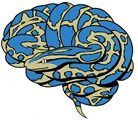
\includegraphics[width=1em]{nipylogo}} % No eye catcher for this poster. (eyecatcher=no above). If an eye catcher is present, the title is centered between eye-catcher and logo.
  % Title
  {\sf %Sans Serif
  %\bf% Serif
  Distributed Neuroimaging Analysis with Nipype and IPython\vspace{0.15em}}
  % Authors
  {\sf %Sans Serif
  % Serif
  Satrajit Ghosh$^1$, Brian Granger$^2$, Fernando Perez$^3$\\
  \small\sf$^1$MIT, Cambridge, MA $^2$California Polytechnic State
  University, San Luis Obispo, CA $^3$University of California,
  Berkeley, CA}


  % University logo
  % {% The makebox allows the title to flow into the logo, this is a hack because of the L shaped logo.
  %   \makebox[8em][r]{%
  %     \begin{minipage}{16em}
  %       \hfill
  %       %\includegraphics[height=2em]{msrlogo}
  %       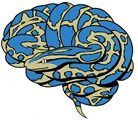
\includegraphics[height=7.0em]{nipylogo}
  %     \end{minipage}
  %   }
  % }

  \tikzstyle{light shaded}=[top color=baposterBGtwo!30!white,bottom color=baposterBGone!30!white,shading=axis,shading angle=30]

  % Width of left inset image
     \setlength{\leftimgwidth}{0.78em+8.0em}

%%%%%%%%%%%%%%%%%%%%%%%%%%%%%%%%%%%%%%%%%%%%%%%%%%%%%%%%%%%%%%%%%%%%%%%%%%%%%%
%%% Now define the boxes that make up the poster
%%%---------------------------------------------------------------------------
%%% Each box has a name and can be placed absolutely or relatively.
%%% The only inconvenience is that you can only specify a relative position 
%%% towards an already declared box. So if you have a box attached to the 
%%% bottom, one to the top and a third one which should be in between, you 
%%% have to specify the top and bottom boxes before you specify the middle 
%%% box.
%%%%%%%%%%%%%%%%%%%%%%%%%%%%%%%%%%%%%%%%%%%%%%%%%%%%%%%%%%%%%%%%%%%%%%%%%%%%%%
    %
    % A coloured circle useful as a bullet with an adjustably strong filling
   \newcommand{\colouredcircle}[1]{%
      \tikz{\useasboundingbox (-0.2em,-0.32em) rectangle(0.2em,0.32em); \draw[draw=black,fill=headerFontColor!80!black!#1!white,line width=0.03em] (0,0) circle(0.18em);}}
    \renewcommand{\labelitemi}{\colouredcircle{100}}
    \renewcommand{\labelitemii}{\colouredcircle{50}}

%%%%%%%%%%%%%%%%%%%%%%%%%%%%%%%%%%%%%%%%%%%%%%%%%%%%%%%%%%%%%%%%%%%%%%%%%%%%%%
  \headerbox{Introduction}{name=introduction,column=0,row=0}{
%%%%%%%%%%%%%%%%%%%%%%%%%%%%%%%%%%%%%%%%%%%%%%%%%%%%%%%%%%%%%%%%%%%%%%%%%%%%%%
    \begin{list}{\labelitemi}{\leftmargin=1em}
      \compresslist
    \item \textbf{Data explosion.} We face an explosion in the size and
      complexity of neuroimaging datasets, whose analysis not only
      requires sophisticated algorithms but computational infrastructure
      to support their use with ease, efficiency, reliability and
      reproducibility.
   \item \textbf{Limited infrastructure} While existing analysis
      packages provide excellent tools, they often constrain users to
      specific workflows and environments. Furthermore, very few of the
      available neuroimaging tools take advantage of the growing number
      of parallel hardware configurations (multicore, clusters, clouds
      and supercomputers).
   \item \textbf{Nipype+IPython.} We present distributed execution of neuroimaging analysis
      pipelines that the open source Nipype \cite{ghos.python-based.09}
      project has developed by integrating with IPython's
      \cite{pere.ipython.07}.
   \end{list}
   \vspace{-0.3em}
}


%%%%%%%%%%%%%%%%%%%%%%%%%%%%%%%%%%%%%%%%%%%%%%%%%%%%%%%%%%%%%%%%%%%%%%%%%%%%%%
  \headerbox{Features}{name=features,column=0,below=introduction}{
%%%%%%%%%%%%%%%%%%%%%%%%%%%%%%%%%%%%%%%%%%%%%%%%%%%%%%%%%%%%%%%%%%%%%%%%%%%%%%
    \begin{list}{\labelitemi}{\leftmargin=1em}
      \compresslist
      \item Parallel execution of complex workflows.
      \item No additional user code required for parallel execution.
      \item Embarassingly parallel execution supported for wrapped
        interface (currently supports SPM, FSL, FreeSurfer)
      \item Automatic load balancing across cluster.
      \item Multiple protocols for parallel communication.
   \end{list}
   \vspace{-0.3em}}

%%%%%%%%%%%%%%%%%%%%%%%%%%%%%%%%%%%%%%%%%%%%%%%%%%%%%%%%%%%%%%%%%%%%%%%%%%%%%%
  \headerbox{Nipype}{name=nipype,column=1,row=0}{
%%%%%%%%%%%%%%%%%%%%%%%%%%%%%%%%%%%%%%%%%%%%%%%%%%%%%%%%%%%%%%%%%%%%%%%%%%%%%%
    \begin{list}{\labelitemi}{\leftmargin=1em}
      \compresslist
    \item \textbf{Software explosion.} Current neuroimaging software
      offer users various ways to analyze their data. However, this has
      resulted in a heterogeneous collection of specialized applications
      without transparent interoperability or a uniform operating
      interface.
   \item \textbf{Uniform interface.} Nipype, an open-source,
      community-developed initiative under the umbrella of Nipy
      \cite{bret.nipy.09}, solves these issues by providing a uniform
      interface to existing neuroimaging software and by facilitating
      interaction between these packages using workflows.
   \item \textbf{Workflow-based analysis.} Nipype provides an
      environment that not only encourages interactive exploration of
      algorithms, but simplifies the design and execution of
      neuroimaging analysis workflows.
    \end{list}
    \vspace{-0.3em}
  }

%%%%%%%%%%%%%%%%%%%%%%%%%%%%%%%%%%%%%%%%%%%%%%%%%%%%%%%%%%%%%%%%%%%%%%%%%%%%%%
  \headerbox{IPython: Interactive Python}{name=ipython,column=2,row=0}{
%%%%%%%%%%%%%%%%%%%%%%%%%%%%%%%%%%%%%%%%%%%%%%%%%%%%%%%%%%%%%%%%%%%%%%%%%%%%%%
    An \textbf{enhanced interactive Python shell} and \textbf{an architecture
      for interactive parallel computing}.

    IPython provides high-level components to express different parallel
    workflows.  An \emph{IPython Cluster} consists of one or more
    \emph{engines} and one \emph{controller}; code and data can be sent between
    them and multiple \emph{clients} can (even simultaneously) interact:


    \begin{center}
      \begin{tikzpicture}[x=\linewidth,y=\linewidth]
        % \path [use as bounding box] (-0.5,-0.5) rectangle(2.5,1.7);
        \node{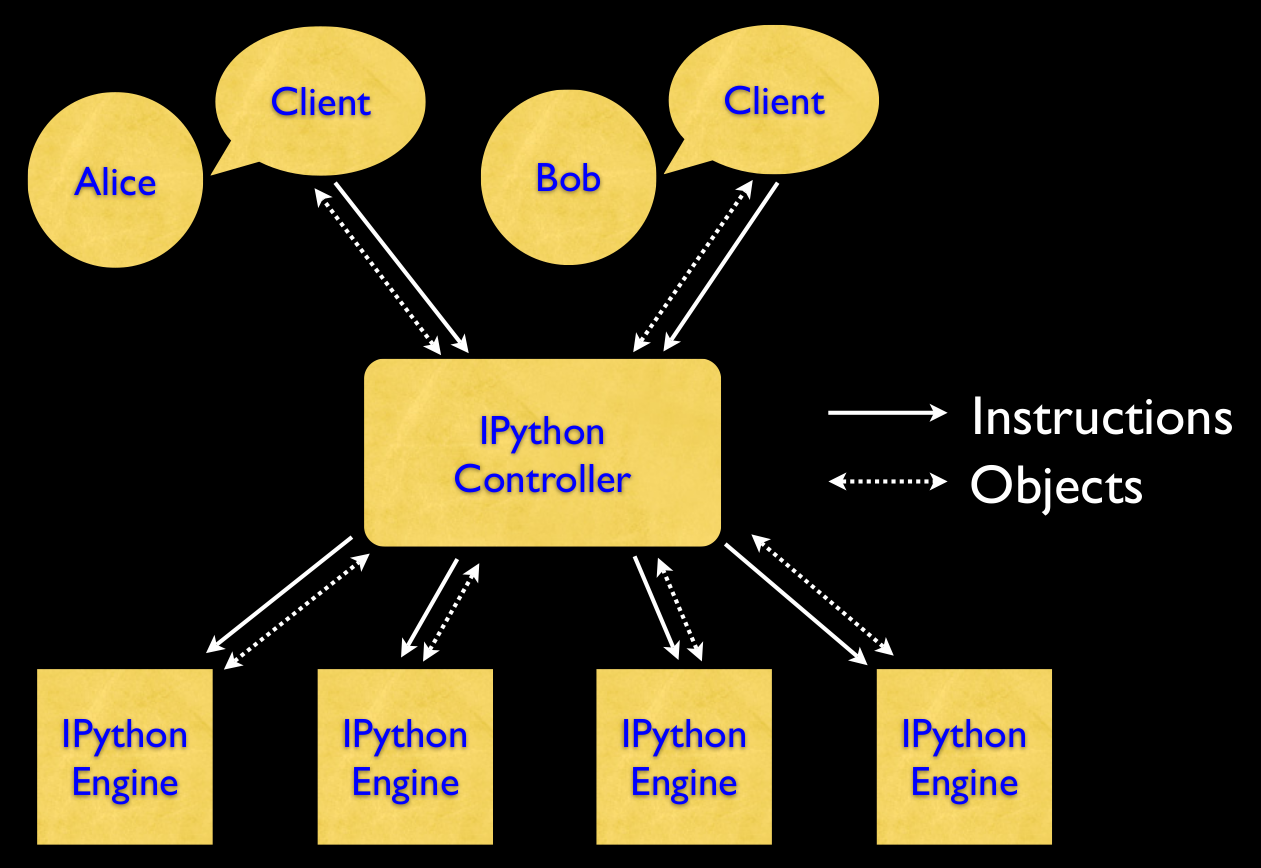
\includegraphics[width=2in]{ipython_dist_architecture}};
      \end{tikzpicture}
    \end{center}

\vspace{0.5em}
  }

%%%%%%%%%%%%%%%%%%%%%%%%%%%%%%%%%%%%%%%%%%%%%%%%%%%%%%%%%%%%%%%%%%%%%%%%%%%%%%
% Setup verbatim environments to create code boxes
%%%%%%%%%%%%%%%%%%%%%%%%%%%%%%%%%%%%%%%%%%%%%%%%%%%%%%%%%%%%%%%%%%%%%%%%%%%%%%
\begin{SaveVerbatim}{IWorkflowImport}
In [1]: from glob import glob
In [2]: import os
In [3]: from IPython.kernel import client
In [4]: from IPython.kernel.client import StringTask
In [5]: from nipype.interfaces.spm import Normalize
\end{SaveVerbatim}

\begin{SaveVerbatim}{IWorkflowSetup}
In [6]: taskstr = """import os
   ...: script_dir = 'script_dir/subj_%d'
   ...: os.makedirs(script_dir)
   ...: os.chdir(script_dir)
   ...: result = node.run(source='%s')"""
In [7]: node = Normalize(template='/templates/T2.nii')
In [8]: tc = client.TaskClient()
In [9]: fl = glob(os.path.abspath('SAD*.nii'))
\end{SaveVerbatim}

\begin{SaveVerbatim}{IWorkflowRun}
In [10]: ids = [tc.run(StringTask(taskstr%(i,f),
   ....:        push=dict(node=node),pull=['result']))
   ....:        for i, f in enumerate(fl)]
\end{SaveVerbatim}

%%%%%%%%%%%%%%%%%%%%%%%%%%%%%%%%%%%%%%%%%%%%%%%%%%%%%%%%%%%%%%%%%%%%%%%%%%%%%%
  \headerbox{Direct distribution}{name=iworkflow2,column=2,below=nipype}{
%%%%%%%%%%%%%%%%%%%%%%%%%%%%%%%%%%%%%%%%%%%%%%%%%%%%%%%%%%%%%%%%%%%%%%%%%%%%%%
    \textbf{Import components}
    \vspace{-0.3em}
    \UseVerbatim[fontsize=\relsize{-2.5}]{IWorkflowImport}
    \vspace{-0.3em}
    \textbf{Setup variables}
    \vspace{-0.3em}
    \UseVerbatim[fontsize=\relsize{-2.5}]{IWorkflowSetup}
    \vspace{-0.3em}
    \textbf{Run in parallel}
    \vspace{-0.3em}
    \UseVerbatim[fontsize=\relsize{-2.5}]{IWorkflowRun}
}

\begin{SaveVerbatim}{IWorkflow1Import}
In [1]: from glob import glob
In [2]: import os
In [3]: from nipype.interfaces.spm import Normalize
In [4]: from nipype.pipeline.engine import (Workflow, 
                                            Node)
\end{SaveVerbatim}

\begin{SaveVerbatim}{IWorkflow1Setup}
In [5]: fl = glob(os.path.abspath('SAD*.nii'))
In [6]: normalize = Node(Normalize(template= \
                                '/templates/T2.nii'),
   ...:                  name='normalize')
In [7]: normalize.iterables = ('source', fl)
In [8]: normworkflow = Workflow(name='normalizefa',
   ...:                    base_dir='./norm_workdir')
In [9]: normworkflow.add_nodes([normalize])
\end{SaveVerbatim}

\begin{SaveVerbatim}{IWorkflow1Run}
In [10]: normworkflow.run()
\end{SaveVerbatim}

%%%%%%%%%%%%%%%%%%%%%%%%%%%%%%%%%%%%%%%%%%%%%%%%%%%%%%%%%%%%%%%%%%%%%%%%%%%%%%
  \headerbox{Indirect distribution}{name=iworkflow1,column=1,below=nipype}{
%%%%%%%%%%%%%%%%%%%%%%%%%%%%%%%%%%%%%%%%%%%%%%%%%%%%%%%%%%%%%%%%%%%%%%%%%%%%%%
    \textbf{Import components}
    \vspace{-0.3em}
    \UseVerbatim[fontsize=\relsize{-2.5}]{IWorkflow1Import}
    \vspace{-0.3em}
    \textbf{Setup variables}
    \vspace{-0.3em}
    \UseVerbatim[fontsize=\relsize{-2.5}]{IWorkflow1Setup}
    \vspace{-0.3em}
    \textbf{Run in parallel}
    \vspace{-0.3em}
    \UseVerbatim[fontsize=\relsize{-2.5}]{IWorkflow1Run}
}

%%%%%%%%%%%%%%%%%%%%%%%%%%%%%%%%%%%%%%%%%%%%%%%%%%%%%%%%%%%%%%%%%%%%%%%%%%%%%%
  \headerbox{Funding}{name=funding,column=1,span=2,above=bottom}{
%%%%%%%%%%%%%%%%%%%%%%%%%%%%%%%%%%%%%%%%%%%%%%%%%%%%%%%%%%%%%%%%%%%%%%%%%%%%%%
    \smaller This project was supported by NIH grants NIBIB R03 EB008673
    (PI: Ghosh, Whitfield-Gabrieli), NIMH R01 MH081909 (PI: D'Esposito).
  }

%%%%%%%%%%%%%%%%%%%%%%%%%%%%%%%%%%%%%%%%%%%%%%%%%%%%%%%%%%%%%%%%%%%%%%%%%%%%%%
  \headerbox{Complex workflows}{name=results,column=1,span=2,below=iworkflow2,above=funding}{
%%%%%%%%%%%%%%%%%%%%%%%%%%%%%%%%%%%%%%%%%%%%%%%%%%%%%%%%%%%%%%%%%%%%%%%%%%%%%%
    \begin{tikzpicture}[x=\linewidth,y=\linewidth]
      \node{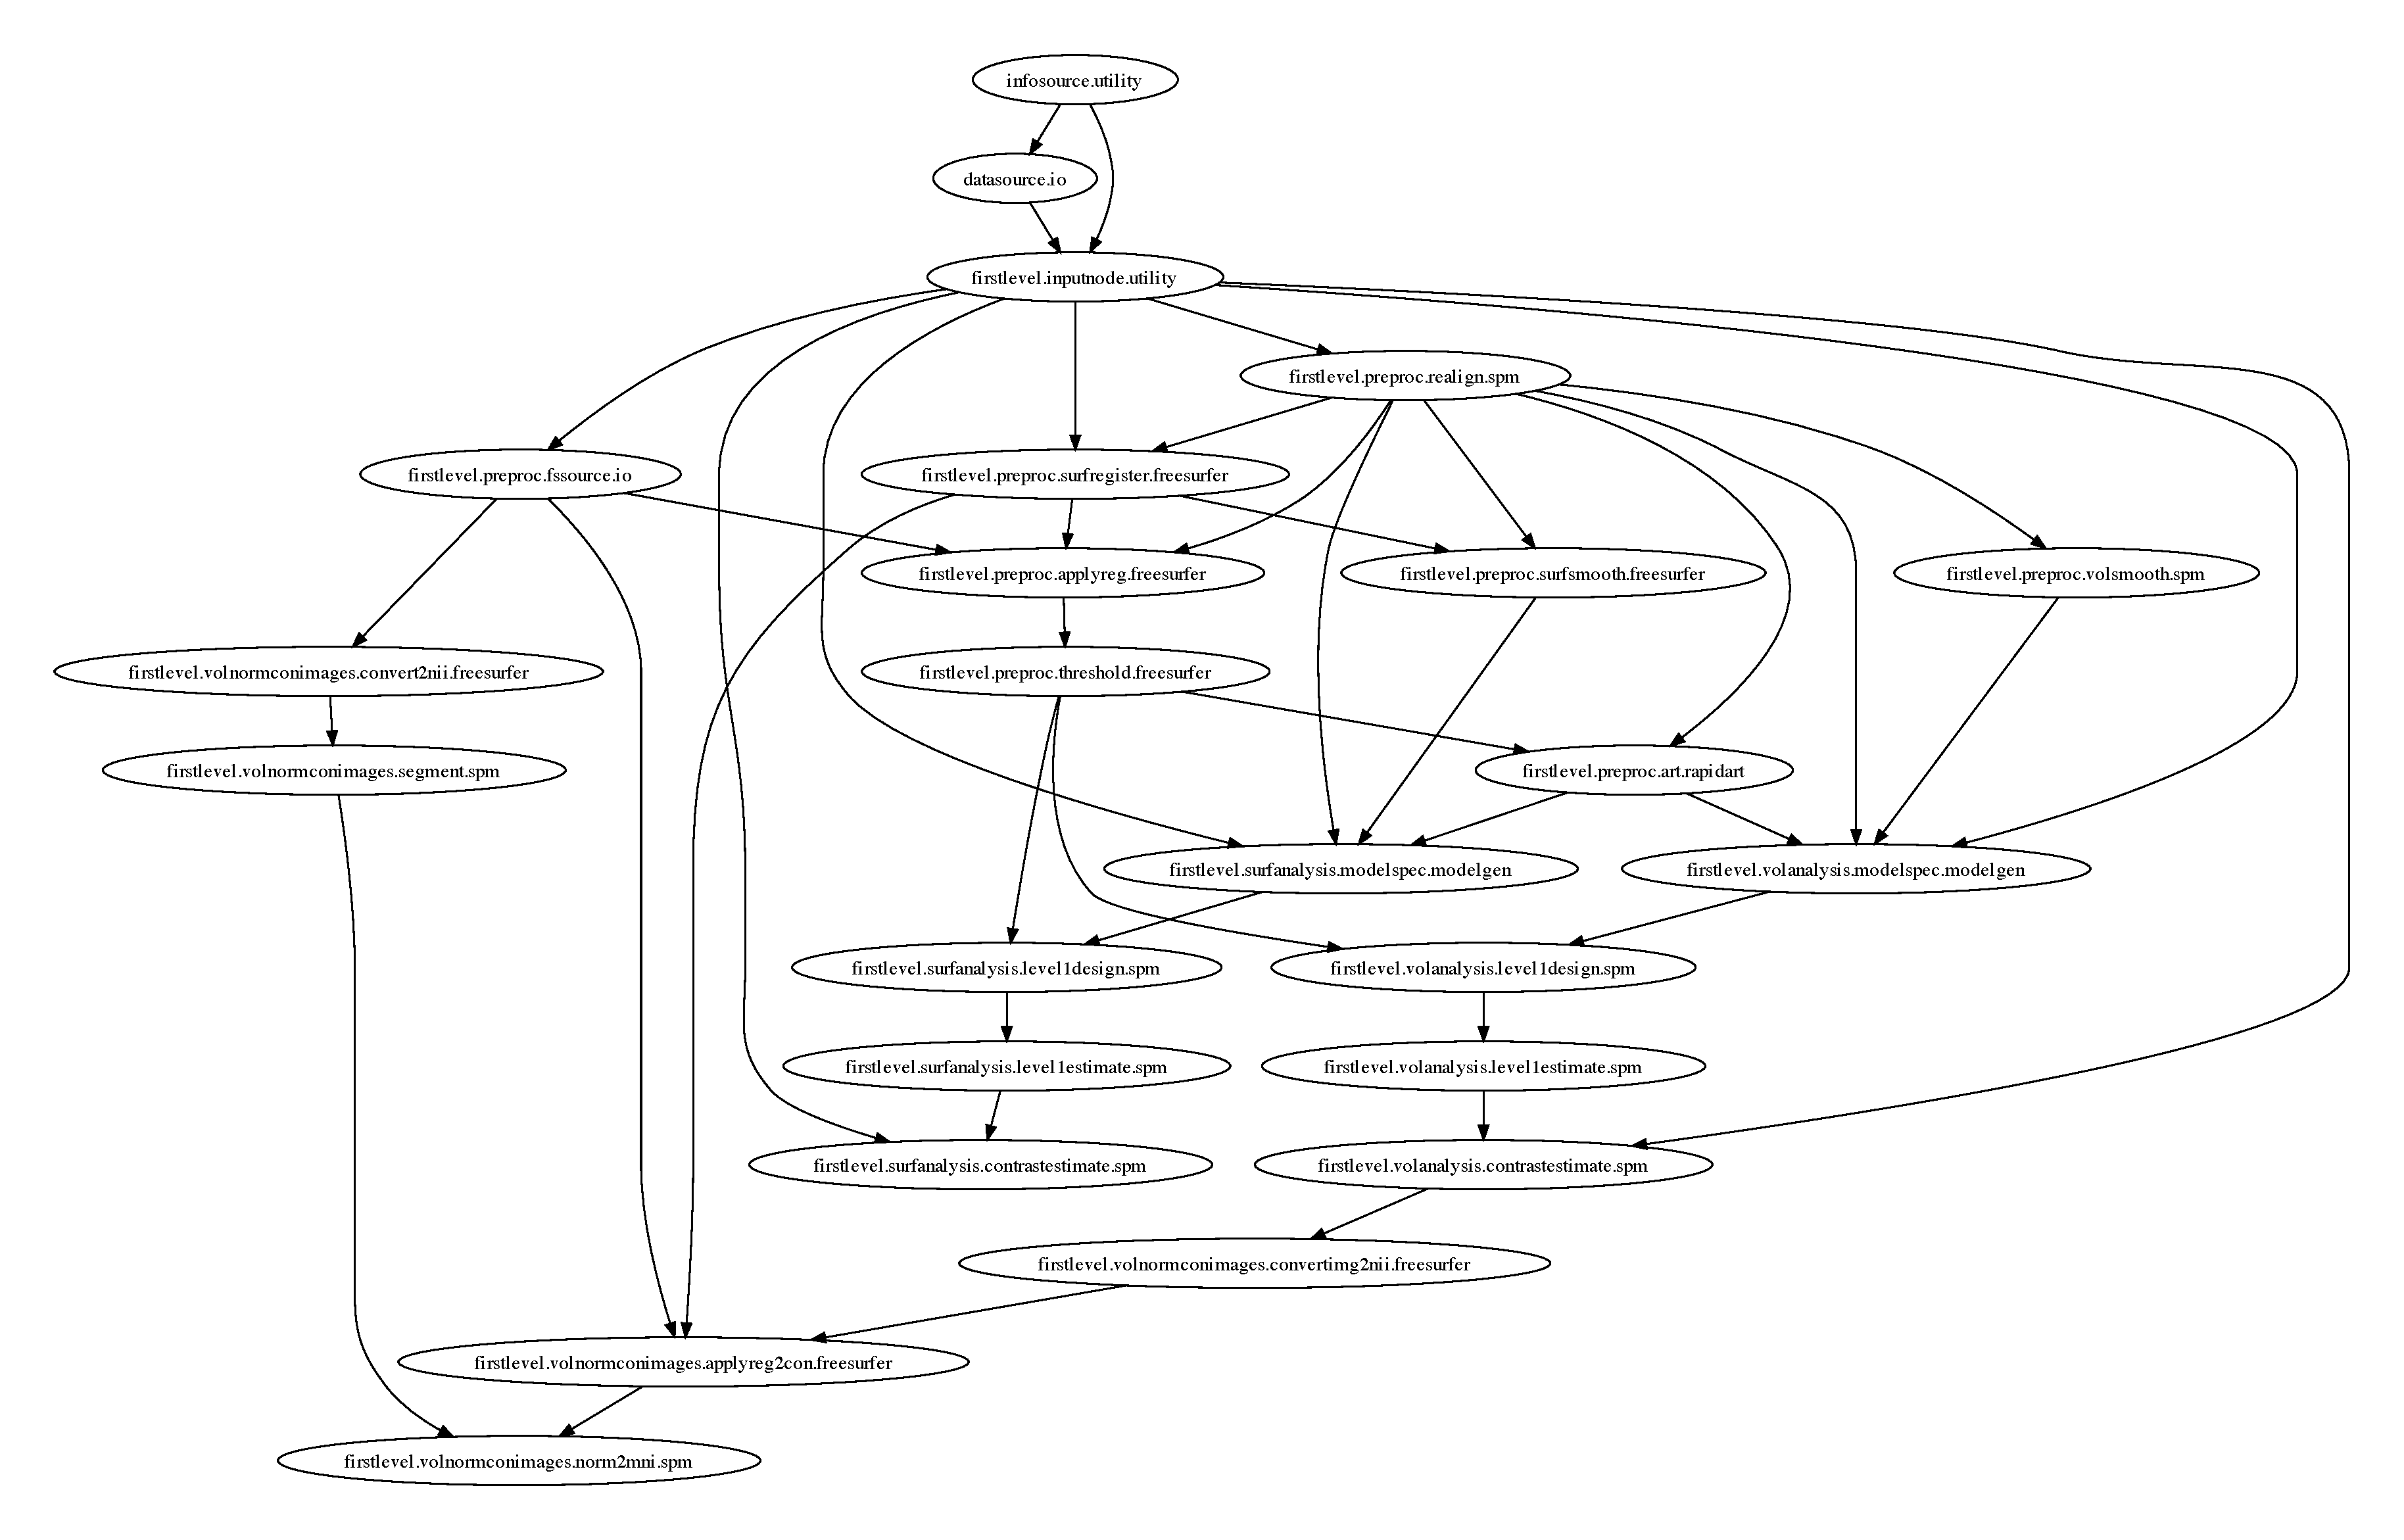
\includegraphics[width=0.8\linewidth]{nipype_graph}};
    \end{tikzpicture}
    \begin{multicols}{2}
     \centering
     Comparative workflow (4 core machine).
     \begin{tabular}{lll}
        serial & 1 subject & 41min\\
        parallel & 1 subject & 25min\\
        parallel & 2 subject & 41min
      \end{tabular}

     SPM workflow (40 core cluster)
     \begin{tabular}{lll}
        serial & 1 subject & 41min\\
        parallel & 1 subject & 25min\\
        parallel & 69 subject & 1 hr 40 min
      \end{tabular}
   \end{multicols}\vspace{-1em}
  }

%%%%%%%%%%%%%%%%%%%%%%%%%%%%%%%%%%%%%%%%%%%%%%%%%%%%%%%%%%%%%%%%%%%%%%%%%%%%%%
  \headerbox{References}{name=references,column=0,above=bottom}{
%%%%%%%%%%%%%%%%%%%%%%%%%%%%%%%%%%%%%%%%%%%%%%%%%%%%%%%%%%%%%%%%%%%%%%%%%%%%%%
    \footnotesize
    \vspace{-0.4em}
    \bibliographystyle{ieee}
    \renewcommand{\section}[2]{\vskip 0.05em}
    \bibliography{poster}
 }

%%%%%%%%%%%%%%%%%%%%%%%%%%%%%%%%%%%%%%%%%%%%%%%%%%%%%%%%%%%%%%%%%%%%%%%%%%%%%%
  \headerbox{Future plans}{name=future,column=0,below=features}{
%%%%%%%%%%%%%%%%%%%%%%%%%%%%%%%%%%%%%%%%%%%%%%%%%%%%%%%%%%%%%%%%%%%%%%%%%%%%%% 
    \begin{list}{\labelitemi}{\leftmargin=1em}
      \compresslist
    \item \textbf{IPython DAG support.} Moving the DAG scheduler to
      IPython itself for efficient load balancing
    \item \textbf{Dataserver-centric parallelization.} Replace Nipype
      controller with data-server (e.g., XNAT) -controlled, file-system
      independent execution.
    \item \textbf{Intelligent routing.} Processes will be routed based
      on their attributes (e.g., OS specificity, software availability)
      or user requirements (e.g., time, funding).
   \end{list}
   \vspace{-0.3em}
}

%%%%%%%%%%%%%%%%%%%%%%%%%%%%%%%%%%%%%%%%%%%%%%%%%%%%%%%%%%%%%%%%%%%%%%%%%%%%%%
  \headerbox{Conclusion}{name=conclusion,column=0,span=1,below=future,above=references}{
%%%%%%%%%%%%%%%%%%%%%%%%%%%%%%%%%%%%%%%%%%%%%%%%%%%%%%%%%%%%%%%%%%%%%%%%%%%%%%
    \begin{list}{\labelitemi}{\leftmargin=1em}
      \compresslist
    \item \textbf{Integration.} Integrated IPython's parallel and
      distributed computing capabilities into Nipype's pipeline
      execution machinery.
    \item \textbf{Codeless parallelization.} Nipype interfaces can be
      parallelized without explicit parallel programming.
    \item \textbf{Multi-package support.} Current support for a variety
      of SPM, FSL and FreeSurfer functions. Available on different
      distributed computing architectures that share a common
      file-system and have these pacakges installed.
    \end{list}
    \vspace{-0.3em}
}

\end{poster}%
\end{document}
